\chapter{Obbiettivi}\label{chapter:obbiettivi}
%%% Descrivo la situazione di partenza ovvero
%%% spiego ciò che abbiamo a disposizione con immagini ovvero configurazione chiusa e aperta
%%% inserisco che come primo obbiettivo ci siamo posti quello di creare uno shortest path non guidato
%%% poi abbiamo deciso di includere la funzione d'energia per guidare la ricerca
%%% le motivazioni che ci hanno spinto a fare questo lavoro --> Capisci come esprimerle
Come spiegato nel precedente capitolo il caso di studio su cui ci focalizziamo e incentriamo il nostro lavoro è la glicoproteina spike del SARS-CoV-2. Focalizziamo la nostra attenzione su questa proteina per studiarne il comportamento attraverso l'uso di tecniche di ricerca locale, avvicinandosi molto alle tecniche di dinamica e modellistica molecolare. Queste due tecniche introdotte si basano su metodi teorici o tecniche computazionali utilizzate per simulare il comportamento delle molecole. Queste tecniche vengono utilizzate per studiare la dinamica di evoluzione nel tempo di un sistema chimico e svolgere il processo mediante l'utilizzo della tecnologia permette l'applicazione della modellistica a sistemi relativamente complessi. Il livello di dettaglio che si può ottenere utilizzando questi sistemi è il livello atomistico; il più piccolo livello di informazione rappresentato dagli atomi individuali (o piccoli gruppi di atomi). Queste tecniche vengono utilizzate per svariati compiti dal folding proteico, la catalisi enzimatica, la stabilità delle proteine, i cambiamenti conformazionali associati alla funzione biomolecolare e il riconoscimento molecolare delle proteine. 
Le tecniche descritte in precedenza hanno però delle problematiche a partire dalle risorse necessarie a compiere questo tipo di compiti, il tempo computazionale necessario e il fatto che si possa lavorare in modo completo solo su piccole strutture oppure è necessario limitare di molto lo spazio di lavoro. 
 
Ricollegandoci alla Glicoproteina spike del SARS-CoV-2 prendiamo in considerazione entrambe le configurazioni sia quello in stato chiuso che quella in stato aperto; esse differiscono per lo stato in cui si trova la parte mobile: nella chiusa si trova in uno stato di pre fusione; nello stato aperto è pronta a legarsi ad un recettore. Possiamo vedere realmente la differenza delle due configurazioni guardando la Fig. \ref{fig:Configurazioni}.  

\begin{figure}
	\centering
	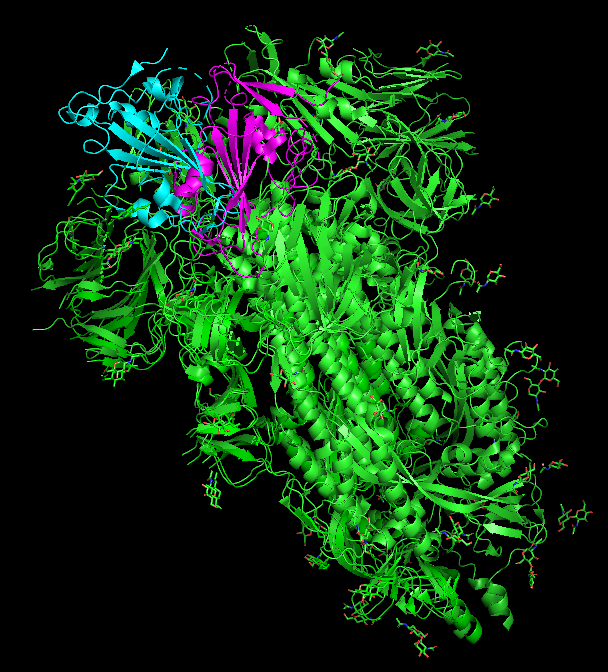
\includegraphics[width=0.6\textwidth]{Immagini/Struttura_aperta_chiusa.png}
	\caption{La Glicoproteina spike nelle due configurazioni: contraddistinta dal colore magenta troviamo la configurazione chiusa; contraddistinta dal colore ciano troviamo la configurazione aperta.}
	\label{fig:Configurazioni}
\end{figure}

L'obbiettivo di questo framework lavorando sulle due configurazione della glicoproteina spike del SARS-CoV-2 è quello di trovare uno shortest path tra le due configurazioni utilizzando due principi differenti per il costo del singolo movimento.
\vspace{10pt}
\begin{itemize}
	\item calcolo del costo mediante la sola geometria, ovvero somma delle componenti di traslazione e angolo di rotazione 
	\vspace{5pt}
	\item calcolo del costo mediante non solo la geometria, ma l'utilizzo della funzione d'energia per minimizzare le variazioni di energia. 
\end{itemize}

Il percorso più breve porta con se la necessità di ottenere delle configurazioni intermedie per raggiungere l'obbiettivo preposto e questo ci porta a dover affrontare il problema della fattibilità della connessione tra parte mobile nella nuova configurazione e la parte fissa [Fig. \ref{fig:Dettaglio} ]. In questo caso si va effettivamente ad agire sugli amminoacidi che fanno parte dei due loop che collegano appunto le parti e in questo caso possiamo affermare che il framework proposto si occupa non solo del movimento della backbone (catena principale), ma tiene in considerazione anche la presenza delle catene laterali. Le catene laterali non vengono coinvolte attivamente nel movimento, ma viene considerato l'ingombro nei confronti e nel rispetto delle proprietà chimico-fisiche. Il framework quindi muove la catena principale rispettando la struttura dell'amminoacido e poi nel rispetto della struttura si preoccupa che la catena laterale non effettui clash con nessun amminoacido nelle vicinanze. 

\begin{figure}
	\centering
	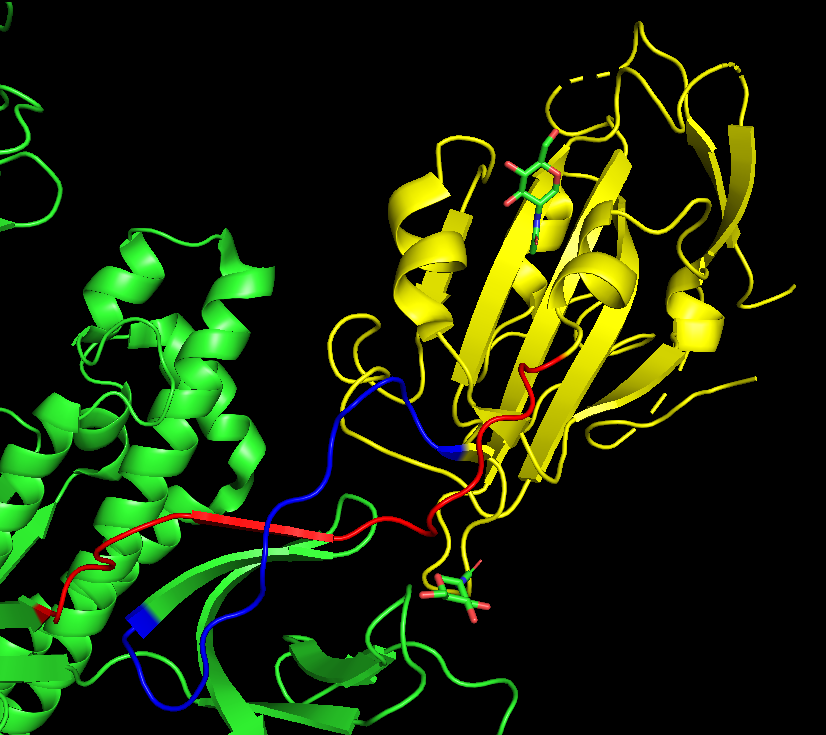
\includegraphics[width=0.6\textwidth]{Immagini/Struttura_spike_dettaglio.png}
	\caption{Nell'immagine dettagliata notiamo i due loop che collegano la parte mobile alla parte fissa colorati rispettivamente di rosso e di blu.}
	\label{fig:Dettaglio}
\end{figure}

Il motivo per cui è stato effettuato questo lavoro è quello di proporre un framework che fosse in grado di fornire un metodo per lo studio del movimento di una proteina in modo più ampio rispettando comunque tutte le regole necessarie in questo tipo di movimenti. Questo framework consente quindi di effettuare studi di più larga scala rispetto a quanto fornito dai metodi di dinamica molecolare e giocando con i parametri che tengono in considerazione il clash possiamo fornire uno strumento con complessità computazionale minore. 

